

\fancypagestyle{miEstilo4}{
   \lhead{4. Tecnologías y herramientas usadas}
   %\chead{1. Introducción}
   \rhead{Página \thepage}
   \lfoot{}
   \cfoot{}
   \rfoot{}
}

\pagestyle{miEstilo4}

\section{Tecnologías y herramientas utilizadas}

Para el desarrollo de este proyecto se han utilizado una gran cantidad de herramientas y tecnologías de código abierto. A continuación se muestra cada una de ellas.

\subsection{Diseño}

Para el diseño de este proyecto, se han realizado prototipos y diagramas para poder diseñar la arquitectura y principales componentes de la aplicación, además de la interacción de los componentes con el resto. Para realizar esto, se ha utilizado el siguiente software:

\textbf{Draw.io}

Draw.io \cite{ref7} es una aplicación para diseño y diagramas de aplicaciones. Es un servicio gratis de Google y de código abierto.

Este software se ha utilizado para diagramas de diseño de interfaz.

\begin{figure}[h]
	\centering
	
\includegraphics[scale=0.5]{images/4}
\end{figure}

\textbf{Visual paradigm} 

Visual paradigm \cite{ref8}  es un software de modelado UML que nos permite analizar, diseñar,
codificar, probar y desplegar. Dibuja todo tipo de diagramas UML, genera código fuente a
partir de dichos diagramas y también posibilita la elaboración de documentos.


\begin{figure}[h]
	\centering
	
\includegraphics[scale=0.5]{images/5}
\end{figure}

Este software se ha utilizado para la generación del diagrama de clases e interacción entre componentes.

\newpage

\subsection{Sistema control de versiones}

Los sistemas de control de versiones \cite{ref9} son programas que tienen como objetivo controlar los cambios en el desarrollo de cualquier tipo de software, permitiendo conocer el estado actual de un proyecto, los cambios que se le han realizado a cualquiera de sus piezas, las personas que intervinieron en ellos \ldots

El control de versiones es una de las tareas fundamentales para la administración de un proyecto de desarrollo de software en general. Surge de la necesidad de mantener y llevar control del código que vamos programando, conservando sus distintos estados. Es absolutamente necesario para el trabajo en equipo, pero resulta útil incluso a desarrolladores independientes. 

Por este motivo, no he dudado en utilizar un sistema de control de versiones. El sistema de control de versiones me ha facilitado mucho la gestión y seguimiento del proyecto. El sitema que he utilizado ha sido \texttt{git}, y como medio de alojamiento para este proyecto he utilizado  \texttt{Github}.

\textbf{Git}

\texttt{Git} \cite{ref10}  es un sistema de control de versiones distribuido, de código libre y multiplataforma que permite la gestión de repositorios software a través de una línea de comandos \cite{ref9}.

Para este proyecto, se ha creado un repositorio donde se ha almacenado todo el código fuente de la aplicación junto con sus cambios a lo largo de su desarrollo.

\begin{figure}[h]
	\centering
	
\includegraphics[scale=0.25]{images/6}
\end{figure}

\textbf{Github}

\texttt{Github} \cite{ref11} es un servicio para alojamiento de repositorios de software gestionados por el sistema de control de versiones \texttt{Git}. En definitiva, \texttt{Github} es un sitio web pensado para hacer posible el compartir el código de una manera más fácil y al mismo tiempo darle popularidad a la herramienta de control de versiones en sí, que es \texttt{Git}.

Este proyecto se ha ido alojando en el repositorio de Github \url{https://github.com/jmv74211/TFM_security_system_PI}.

\begin{figure}[h]
	\centering
	
\includegraphics[scale=0.2]{images/7}
\end{figure}

\subsection{Lenguajes de programación y lenguajes de marcas}

La implementación de este proyecto está desarrollada básicamente en \texttt{Python}. También se ha hecho uso de otros lenguajes de programación para alguna tarea en particular.

A continuación se muestran los lenguajes de programación utilizados.

\textbf{Python}

\texttt{Python} es un lenguaje de programación interpretado, de alto nivel y de propósito general. Este lenguaje de programación viene instalado predeterminadamente en casi todos los sistemas operativos, y consta de un gran número de bibliotecas para realizar una gran cantidad de tareas.

\texttt{Python} se ha utilizado como lenguaje de programación base, con aproximadamente un 90\% del código fuente total. Básicamente he elegido este lenguaje ya que Raspberry PI posee bibliotecas para interaccionar con \texttt{Python}, y con el resto de componentes involucrados.

\begin{figure}[h]
	\centering
	
\includegraphics[scale=0.13]{images/8}
\end{figure}

\textbf{HTML, CSS y Javascript}

Para poder visualizar el streaming de vídeo a través del navegador, ha sido necesario implementar una pequeña página web utilizando \texttt{HTML} y \texttt{CSS}. Respecto a la parte de conexión entre la cámara y el navegador se ha utilizado \texttt{Python} para crear el servidor HTTP y la conexión websocket, y una biblioteca de funciones de \texttt{Javascript} para la transmisión de datos.

\vspace{-0.5cm}

\begin{figure}[h]
	\centering
	
\includegraphics[scale=0.7]{images/9}
\end{figure}

\vspace{-1cm}

\textbf{BASH}

Bash es un intérprete de comandos que ejecuta, una por una, las instrucciones introducidas por el usuario o contenidas en un script y devuelve los resultados. En otras palabras, actúa como interfaz entre el kernel Linux y los usuarios o programas del modo texto. Además, incorpora numerosas utilidades de programación y mejoras sobre sh, su shell predecesora. Debido a que es una herramienta desarrollada por GNU, suele ser utilizada por defecto en las distros actuales.

\begin{figure}[h]
	\centering
	
\includegraphics[scale=0.15]{images/10}
\end{figure}

En este proyecto se ha programado un script en \texttt{bash} para iniciar o parar la aplicación.

\subsection{Bibliotecas y frameworks externos}

Para la implementación de este proyecto, se han utilizado un gran número de bibliotecas para poder interaccionar entre sus distintos componentes.

A continuación se describen brevemente las bibliotecas y frameworks utilizados.

\newpage

\textbf{PiCamera}

\texttt{PiCamera} \cite{ref12} es una biblioteca de \texttt{Python} que proporciona una gran cantidad de funciones para interaccionar directamente con la cámara de la Raspberry PI.

Esta biblioteca ha sido utilizada en los módulos que interactúan directamente con el recurso hardware de la cámara.


\begin{figure}[h]
	\centering
	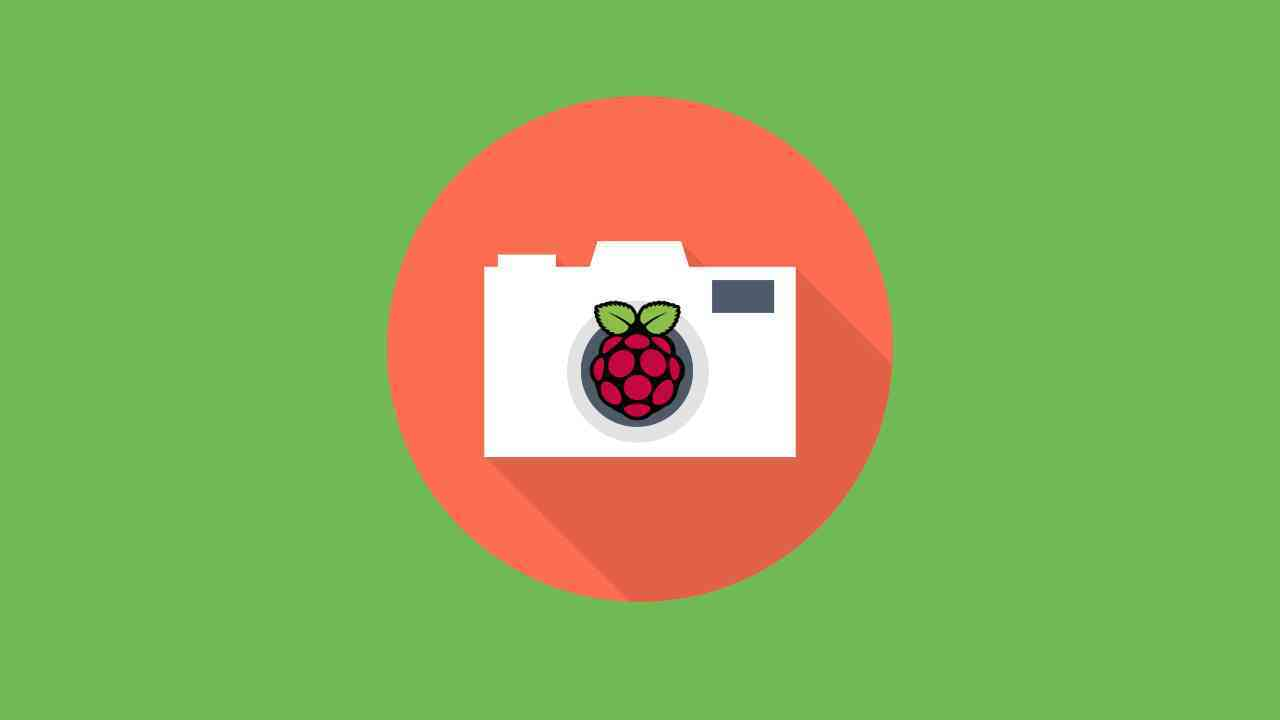
\includegraphics[scale=0.09]{images/11}
\end{figure}

\textbf{pyTelegramBotAPI}

\texttt{pyTelegramBotAPI} \cite{ref13} es una biblioteca de funciones de alto nivel que hace uso de la API de Telegram.

En este proyecto se ha utilizado para crear el bot de Telegram, que será la aplicación con la que el usuario interaccionará, y éste a su vez con la API desarrollada en la aplicación backend.

\begin{figure}[h]
	\centering
	
\includegraphics[scale=0.22]{images/12}
\end{figure}

\textbf{Flask}

\texttt{Flask} \cite{ref14} es un framework ligero de aplicaciones web WSGI. Está diseñado para hacer que el despliegue de una aplicación sea rápida y fácil, con la capacidad de escalar a aplicaciones complejas.

En este proyecto se ha utilizado para implementar varios servicios web, como la API principal que interactúa con el resto de módulos y componentes.

\begin{figure}[h]
	\centering
	
\includegraphics[scale=0.19]{images/13}
\end{figure}

\textbf{Celery}

\texttt{Celery} \cite{ref15} es una implementación de una cola de tareas para aplicaciones web de \texttt{Python} que se utiliza para ejecutar tareas de forma asíncrona.

En este proyecto se ha utilizado principalmente en la API y en el agente de movimiento. El objetivo es poder realizar peticiones, y que la API atienda al mayor número de ellas, devolviendo la respuesta tras la ejecución de las tareas, sin producir ningún tipo de espera entre las comunicaciones (Más información en la sección \ref{sec:composer}).

\vspace{-0.6cm}

\begin{figure}[h]
	\centering
	
\includegraphics[scale=0.15]{images/14}
\end{figure}

\vspace{-1.4cm}

\textbf{RPi.GPIO}

\texttt{RPi.GPIO} \cite{ref16} es un paquete que provee de una clase para controlar las conexiones GPIO de la Raspberry PI.

En este proyecto es usado para recibir la señal del sensor de movimiento, de forma que es posible saber cuándo se ha activado.

\begin{figure}[h]
	\centering
	
\includegraphics[scale=0.15]{images/15}
\end{figure}

\vspace{-0.6cm}

\textbf{Tensorflow}

\texttt{Tensorflow}  es una plataforma de código abierto para aprendizaje automático. Cuenta con un ecosistema completo y flexible de herramientas, bibliotecas y recursos que permiten a los investigadores impulsar el estado del arte en machine learning y a los desarrolladores construir y desplegar fácilmente aplicaciones potenciadas por el machine learning.

En este proyecto se ha utilizado para construir un agente que sea capaz de reconocer objetos en una foto utilizando un modelo ligero preentrenado (más información en la sección \ref{sec:composer}).

\begin{figure}[h]
	\centering
	
\includegraphics[scale=0.12]{images/19}
\end{figure}

\textbf{Requests}

\texttt{Requests} \cite{ref18} es una librería HTTP con licencia Apache2, escrita en \texttt{Python}. Permite enviar peticiones HTTP/1.1, además de añadir cabeceras, datos de formulario, archivos y parámetros con diccionarios \texttt{Python} simples, y acceder a los datos de respuesta de la misma manera.

En este proyecto ha sido utilizado para la comunicación entre los servicios a través de sus API's.

\begin{figure}[h]
	\centering
	
\includegraphics[scale=0.08]{images/20}
\end{figure}

\vspace{-0.5cm}

\subsection{Documentación}

\textbf{LaTeX}

Para elaborar la documentación se ha utilizado \texttt{LaTeX} \cite{ref19} que es un sistema de elaboración de documentos para una composición tipográfica de alta calidad. Se utiliza con mayor frecuencia para documentos técnicos o científicos de mediano a gran tamaño, pero se puede utilizar para casi cualquier forma de publicación.

Para este proyecto se ha utilizado \texttt{LaTeX}, utilizando la distribución \texttt{TEXLive} \cite{ref20} que proporciona un sistema TeX completo con binarios para la mayoría de las versiones de Unix, incluyendo GNU/Linux, macOS, y también Windows. Incluye todos los principales programas relacionados con TeX, paquetes de macros y fuentes que son software libre, incluyendo soporte para muchos idiomas en todo el mundo. 

\begin{figure}[h]
	\centering
	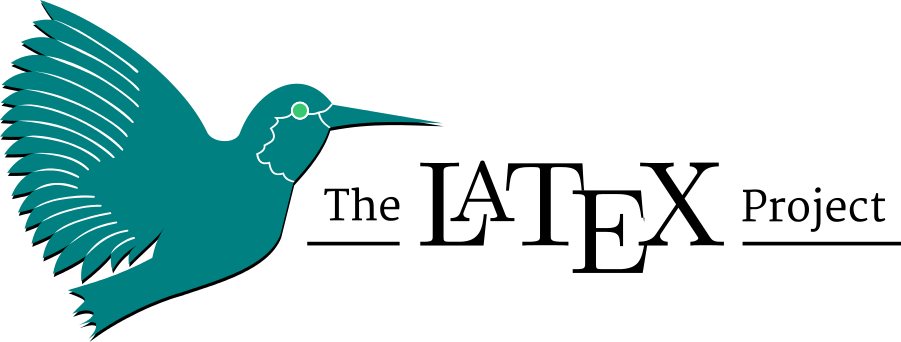
\includegraphics[scale=0.18]{images/16}
\end{figure}

\textbf{TeXstudio}

\texttt{TeXstudio} \cite{ref21} es un entorno integrado para crear documentos LaTeX. El objetivo es conseguir que escribir LaTeX sea lo más fácil y cómodo posible.

Para este proyecto se ha utilizado la versión \textit{2.12.14}.

\begin{figure}[h]
	\centering
	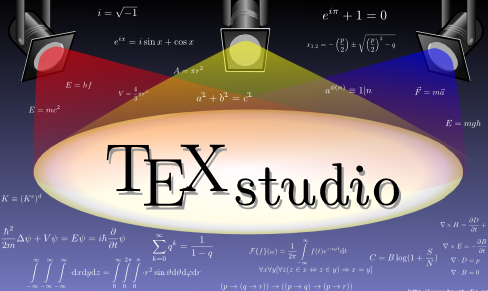
\includegraphics[scale=0.3]{images/17}
\end{figure}

\subsection{Entorno de desarrollo}

El entorno de desarrollo ha sido un aspecto muy importante para la implementación del proyecto, ya que el código se está ejecutando en una Raspberry PI que tiene recursos muy limitados, y los editores o entornos que puede utilizar no son los más cómodos.

Por este motivo, he estado investigando si se puede realizar un desarrollo de la aplicación vía remota. Leyendo foros, observé que el entorno de desarrollo \texttt{pycharm} tiene la opción de poder crear y desarrollar un proyecto vía SSH.

\textbf{Pycharm}

Pycharm \cite{ref22} es un entorno de desarrollo profesional de \texttt{Python}. Gracias a dicho entorno de desarrollo he podido gestionar el proyecto de forma local, ya que los cambios generados se han sincronizado y ejecutado en la Raspberry PI a través de SSH.

En este proyecto se ha utilizado la versión \textit{2019.1.3 Profesional edition}, licencia académica que he obtenido gracias a la UGR. 

\begin{figure}[h]
	\centering
	
\includegraphics[scale=0.06]{images/18}
\end{figure}


\subsection{Otros servicios}

\textbf{Rabbit MQ} 

\texttt{RabbitMQ} \cite{ref23} es un broker de mensajes que acepta y reenvía mensajes. Un broker de mensajes actúa como plataforma intermediaria a la hora de procesar la comunicación entre dos aplicaciones.

En este proyecto ha sido utilizado para crear dos colas de procesos, utilizados por las tareas asíncronas desarrolladas con \texttt{celery}.

\begin{figure}[h]
	\centering
	
\includegraphics[scale=0.2]{images/21}
\end{figure}

\textbf{Telegram bot API} 

Los bots de Telegram \cite{ref24} son aplicaciones de terceros que se ejecutan dentro de Telegram. Los usuarios pueden interactuar con los bots enviándoles mensajes, comandos y peticiones. Se pueden controlar estos bots usando peticiones HTTPS a la API de bot de Telegram.

En este proyecto se ha utilizado para crear un bot de Telegram que interactúe con el usuario y con la aplicación backend desarrollada.

\begin{figure}[h]
	\centering
	
\includegraphics[scale=0.1]{images/22}
\end{figure}


